\documentclass[12pt]{article}
\usepackage[utf8]{inputenc}
\usepackage[left=1.5cm, right=1.5cm, top=2.8cm, bottom=2cm]{geometry}
\geometry{a4paper}
\usepackage{fancyhdr}
\usepackage{pdflscape}
\usepackage{graphicx}

\pagestyle{fancy}
\fancyhf{}
\fancyhead[L]{Labo 8 - Echecs}
\fancyhead[C]{POO}
\fancyhead[R]{V.Cosmo, C. Koestli, S.Roland}
\fancyfoot[C]{\thepage}

\title{
    \vspace{-2cm}
    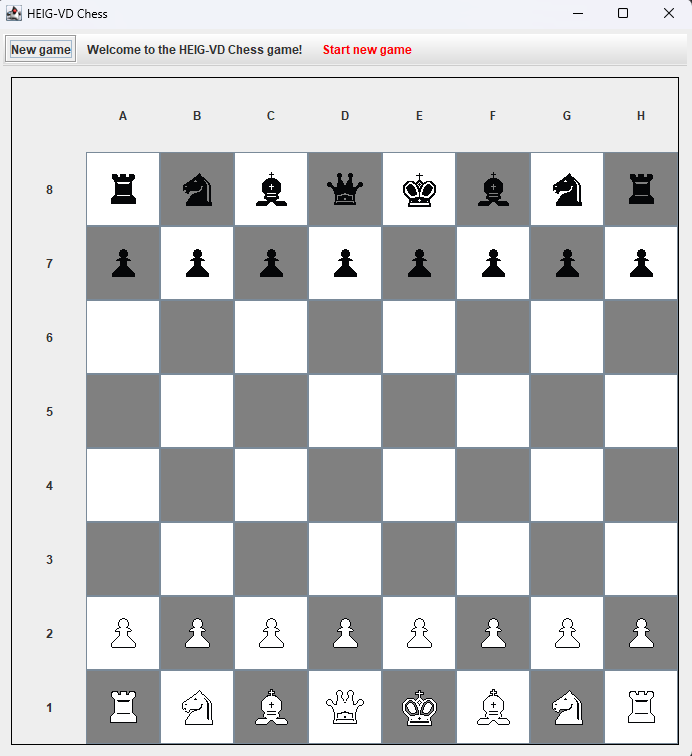
\includegraphics[width=10cm]{chessgame.png} \\
    \Huge{Laboratoire 8} \\
    \Large{Echec}
}
\author{
    Auteurs : \\
    Cosmo de Oliveira Maria Vitória \\
    Koestli Camille \\
    Roland Samuel \\
    \\
    Professeur : \\
    Donini Pier \\
    Assistant : \\
    Decorvet Grégoire
}
\date{
    Classe : A \\
    Date : 10.01.2024
}

\begin{document}

    \maketitle

    \thispagestyle{empty} % No page number on the first page
    \newpage

\maketitle

\section{Introduction}

L'objectif de ce laboratoire est de créer un jeu d'échecs, en respectant certaines règles de bases et sur un interface de jeu. Le jeu est conçu pour être joué en mode console ou avec une interface graphique utilisateur (GUI).

\section{Exécution}

Nous avons migré le projet vers Gradle afin de pouvoir écrire des tests automatisés avec Junit et les lancer en mode continu. Pour lancer le projet, il est possible d'utiliser Gradle.\\
Pour lancer le mode graphique \texttt{gradle run}\\
Pour lancer le mode console: \texttt{gradle run --args="-c" --console plain -q}\\
\\Si vous préférez ne pas installer Gradle, il y a également le wrapper disponible à la racine du dossier. Il suffit de remplacer dans les commandes ci-dessus \texttt{gradle} par \texttt{./gradlew} Linux/Mac ou \texttt{.\textbackslash gradlew} sous Windows.

\section{Explication du Code}

\subsection{Structure Principale}

Nous avons construit notre jeu autour de plusieurs classes clés :

\begin{itemize}
    \item \textbf{Chess}: La classe principale qui lance le jeu. Elle crée le contrôleur (\texttt{ChessController}) et la vue (\texttt{ChessView}), soit en mode console (\texttt{ConsoleView}) soit en mode GUI (\texttt{GUIView}).
    \item \textbf{Board}: Classe qui représente le plateau de jeu. Il gère les pièces sur le plateau, leurs mouvements, et vérifie si un roi est en échec. Nous avons aussi choisir de traiter si le roi est en échec dans cette classe. Le jeu vérifie après chaque mouvement si un roi est en échec, ce qui est crucial pour respecter les règles des échecs. En plus de la liste des pièces dans un tableau 2 dimensions, nous stockons le dernier mouvement et la dernière pièce déplacée afin de valider certaines contraintes de la prise en passant.
    \item \textbf{Piece}: Il s'agit d'une classe abstraite représentant les différentes pièces d'échecs. Chaque type de pièce est une sous-classe de \texttt{Piece}. Cette classe gère les mouvements valides, les collisions, et si une pièce a déjà été déplacée. La pièce connait sa position sur le plateau, cette position est tenue à jour via la méthode \texttt{Piece.setPoint()}, ainsi que son dernier mouvement défini via \texttt{Piece.setLastMove()} permettant de savoir si elle a bougé.
    \item \textbf{Move}: Cette classe représente un mouvement sur le plateau par un vecteur (x,y) et un maximum de fois que l'opération peut être faite, ce qui permet de décrire n'importe quel mouvement. Il contient la logique pour vérifier si un mouvement est valide et pour appliquer les changements sur le plateau. Pour les mouvements spéciaux, nous avons créé différentes sous-classes de \texttt{Move} afin d'y implémenter leurs particularités.
\end{itemize}

\section{Tests réalisés}
Nous avons souhaité réaliser une série de tests qui permettent de vérifier que chaque élément du jeu fonctionne comme prévu. Les tests touchent différents éléments :

\begin{itemize}
    \item \textbf{Tests des mouvements}: Ces tests vérifient la validité des mouvements des pièces sur le plateau. Ils contrôlent que chaque déplacement est conforme aux règles.
    \item \textbf{Tests des conditions d'échec}: Ces tests vont contrôler si le jeu détecte correctement les situations d'échec, c'est-à-dire quand le roi est menacé et empêche tout autre mouvement.
    \item \textbf{Tests du roque}: Ces tests permettent de contrôler que le grand et petit roque ne se produit que lorsque toutes les conditions sont remplies (ni le roi ni la tour n'ont bougé, les cases entre eux sont libres, etc.).
    \item \textbf{Tests de la prise en passant}: Ces tests vérifient que ce mouvement se réalise lorsque le pion adverse a avancé de 2 cases depuis sa position de départ et se trouve à côté du pion attaquant.
    \item \textbf{Tests de la collision}: Ces tests vérifient que les pièves ne peuvent pas se déplacer à travers d'autres pièces, sauf pour le cavalier.

\end{itemize}

\subsection{Tests console}
\paragraph{Méthode:}
Exécution en mode console avec la commande suivante :
\texttt{gradle run --args="-c" --console plain -q}
\\

     \begin{verbatim}
     Start new game
     8 |R N B Q K B N R
     7 |P P P P P P P P
     6 |
     5 |
     4 |
     3 |
     2 |P P P P P P P P
     1 |R N B Q K B N R
     -------------------
        A B C D E F G H
     Next move?
     e2e3
     e2e3
     8 |R N B Q K B N R
     7 |P P P P P P P P
     6 |
     5 |
     4 |
     3 |        P
     2 |P P P P   P P P
     1 |R N B Q K B N R
     -------------------
        A B C D E F G H

     Next move?
     a2a4
     a2a4
     C'est au tour de l'autre joueur...
     Invalid move
     8 |R N B Q K B N R
     7 |P P P P P P P P
     6 |
     5 |
     4 |
     3 |        P
     2 |P P P P   P P P
     1 |R N B Q K B N R
     -------------------
        A B C D E F G H
     Next move?
     a8a6
     a8a6
     Invalid move
     8 |R N B Q K B N R
     7 |P P P P P P P P
     6 |
     5 |
     4 |
     3 |        P
     2 |P P P P   P P P
     1 |R N B Q K B N R
     -------------------
        A B C D E F G H
     Next move?
     a7a5
     a7a5
     8 |R N B Q K B N R
     7 |  P P P P P P P
     6 |
     5 |P
     4 |
     3 |        P
     2 |P P P P   P P P
     1 |R N B Q K B N R
     -------------------
        A B C D E F G H
     Next move?
     \end{verbatim}
Note: nous n'imprimons pas les tests, car cela n'était pas utile et par économie de papiers. Il est bien sûr possible de voir le détail dans le code des tests si besoin dans le rendu Cyberlearn.

\newpage
\subsection{Tests sur les Mouvements}

\begin{table}[h!]
\caption{Tests Move()}
\begin{tabular}{lllll}
\textbf{Pièce}                         & \textbf{Peut aller vers}& \textbf{Et pas vers}                          &  \\
Move de Pion Blanc (1, 1)              & (1, 2)                 & (1, 4), (0, 3), (0, 1), (0, 2), (2, 2), (2, 1) &  \\
Move de Pion Noir (1, 6),              & (1, 5)                 & (2, 5), (2, 4), (3, 4), (1, 3), (0, 5), (1, 7) &  \\
new Move(new Point(2, 1), 3) de (0, 0) & (2, 1), (4, 2), (6, 3) &                                                &  \\
new Move(new Point(0, 1), 1)           & (0, 2),(0, 3),(0, 4)   &                                                &  \\
Move de Knight Blanc (6,0)             & (7, 2)                 & (7, 1), (7, 3)                                 &
\end{tabular}
\end{table}

\begin{table}[h!]
\caption{Tests CastleMove()}
\begin{tabular}{lllll}
\textbf{Nom}                                                                           & \textbf{OK} &  \\
Test du Petit Roque sur roi blanc                                                               & OK &  \\
Test du Grand Roque sur roi blanc                                                               & OK &  \\
Test du Petit Roque sur roi noir                                                                & OK &  \\
Test du Grand Roque sur roi noir                                                                & OK &  \\
Test roque avec des pions qui bloquent le chemin -\textgreater invalide                         & OK &  \\
Test roque ne se produit pas quand le roi a déjà bougé                                          & OK &   \\
Test roque ne se produit pas quand la tour a déjà bougé                                         & OK &   \\
Test grand roque blanc ne se produit pas si on tente de bouger le roi de 3 cases                & OK &  \\
Test de faire un roque avec le roi en échec -\textgreater invalide                              & OK &   \\
Test de faire un roque avec la case intermédiaire menaçée -\textgreater invalide                & OK &   \\
Test de faire un roque alors que le roi est menacé sur la case d'arrivée -\textgreater invalide & OK &
\end{tabular}
\end{table}

\begin{landscape}
\thispagestyle{empty}
\newpage
\section{Diagramme UML}
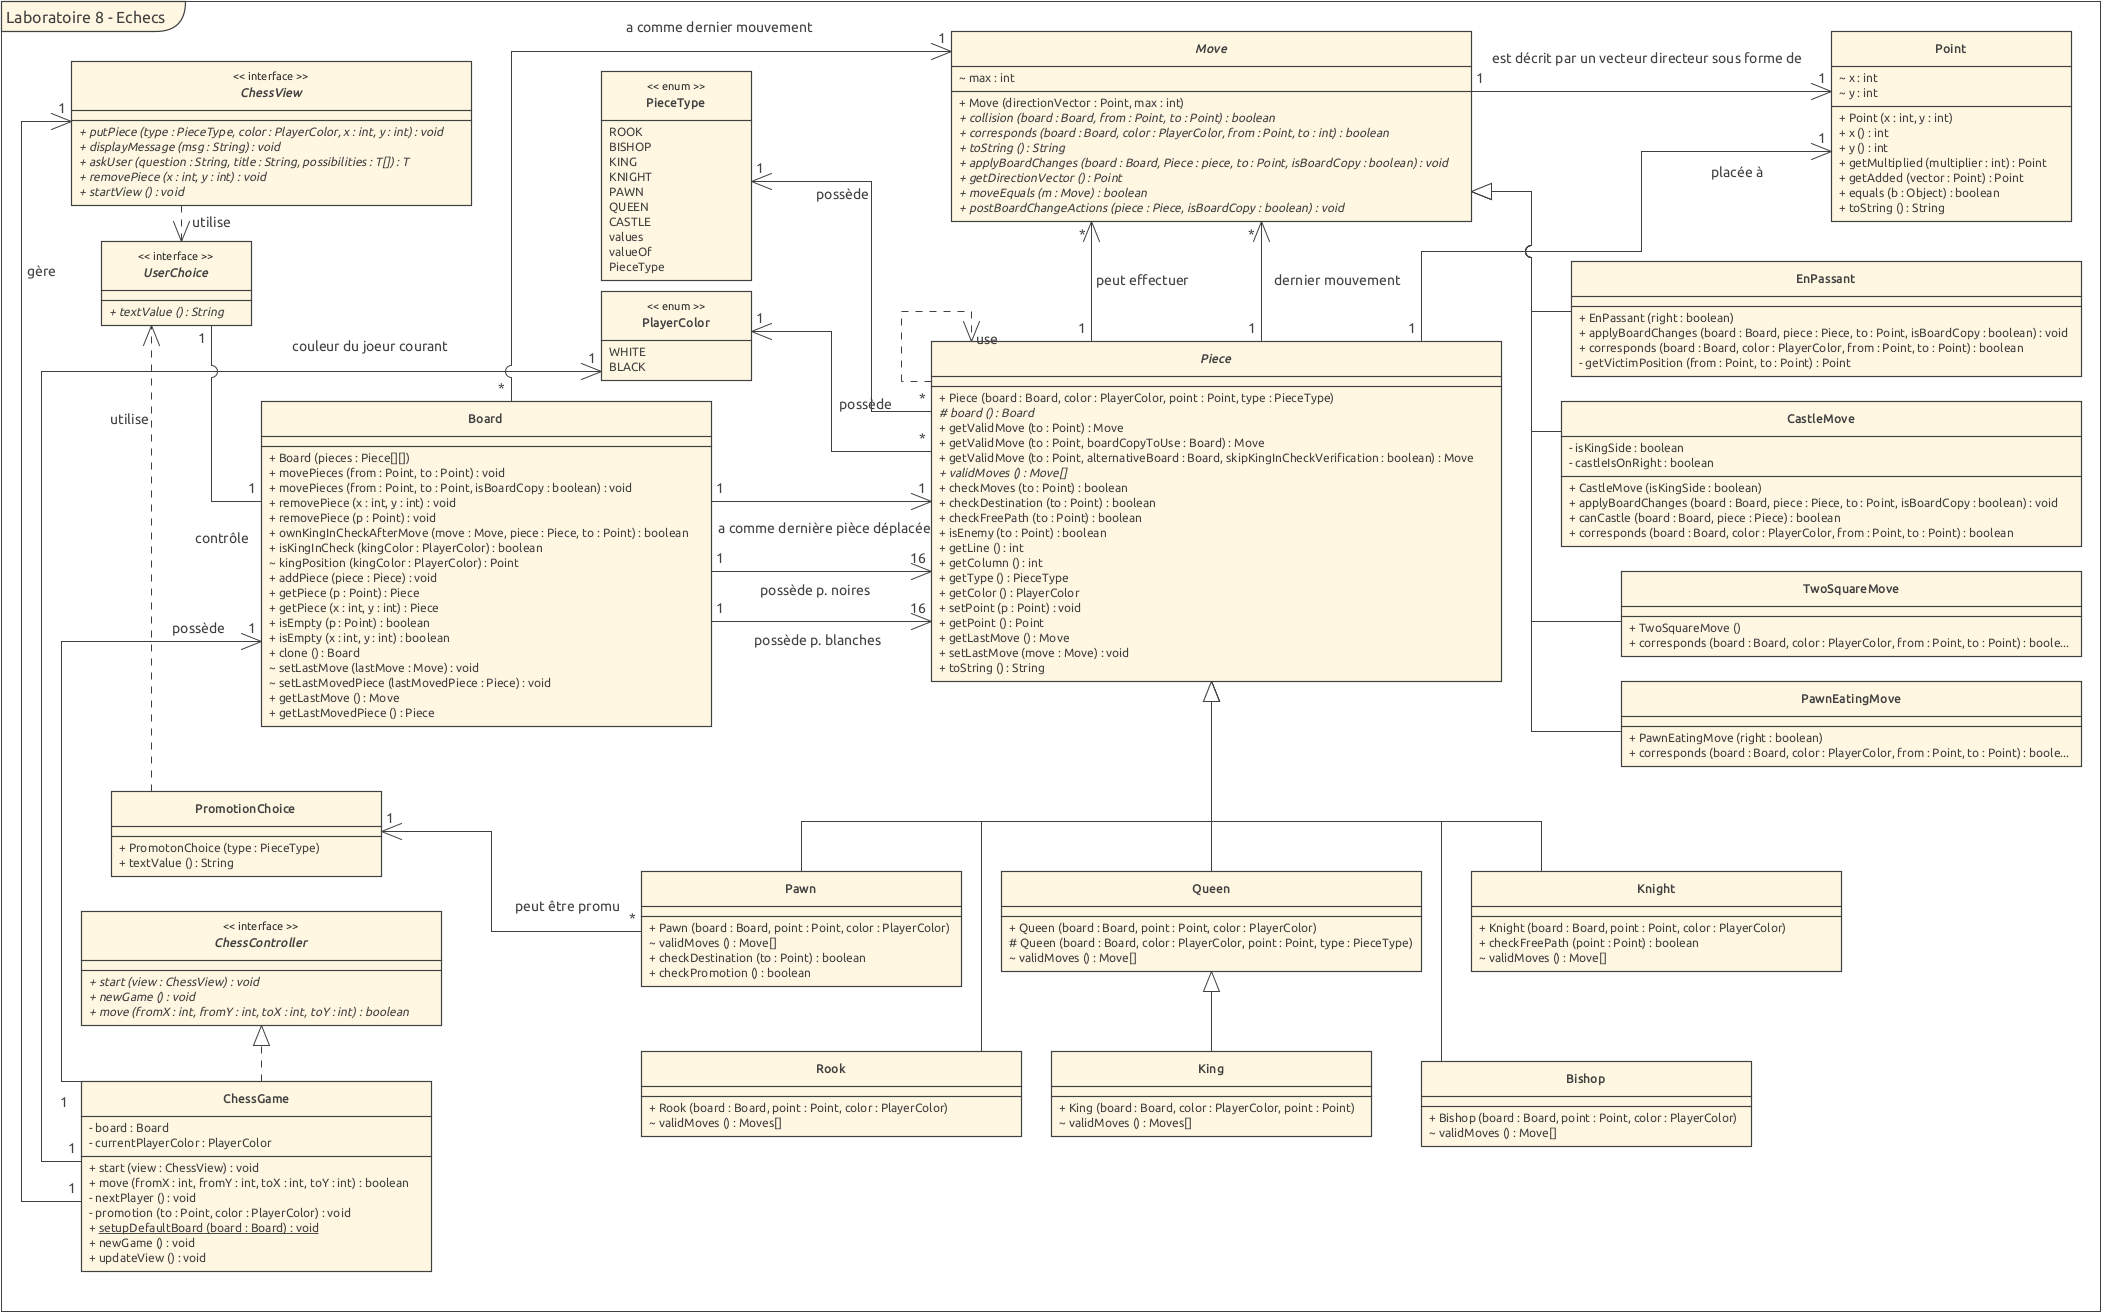
\includegraphics[width=25cm]{uml.png}
\newpage
\end{landscape}

\section{Conclusion}

En conclusion, notre objectif a été de créer un jeu d'échecs en essayant d'être le plus optimisé et complet possible, tout en intégrant les règles de bases. La construction de nos classes a été pensée pour permettre le plus de flexibilité possible. 

Si on imaginait un instant de devoir définir une nouvelle pièce troubadour se déplaçant de 2 cases à gauche ou à droite (une fois sur deux de chaque côté), et qui mange toutes les pièces qu'il touche, il suffirait de créer une classe \texttt{Troubadour} héritant de \texttt{Piece}, de créer un mouvement particulier \texttt{StrangeMove} héritant de \texttt{Move} permettant de détecter la valider que le mouvement droite ou gauche est valide en fonction du dernier mouvement. Une fois le mouvement validé, il reste à implémenter dans \texttt{StrangeMove.applyBoardChanges()} les modifications du plateau à faire en plus du déplacement du troubadourd, c'est à dire de supprimer les pièces qui auraient touchées.

Finalement, nous avons essayé de garantir que notre implémentation puisse s'adapter à certaines modifications de règles restant dans l'esprit du jeu.
\end{document}
